\documentclass[tikz,border=2pt]{standalone}
\usepackage{amsmath}
\usepackage{pgfplots}
\pgfplotsset{compat=1.18}
\usetikzlibrary{arrows.meta}
\begin{document}
% Coercion ladder logical -> integer -> double -> character: a vector takes the most flexible
% type present. Examples: c(TRUE, 1L) integer; c(1L, 1.2), c(TRUE, 1.2) double; c(TRUE, 1L, "a") character.
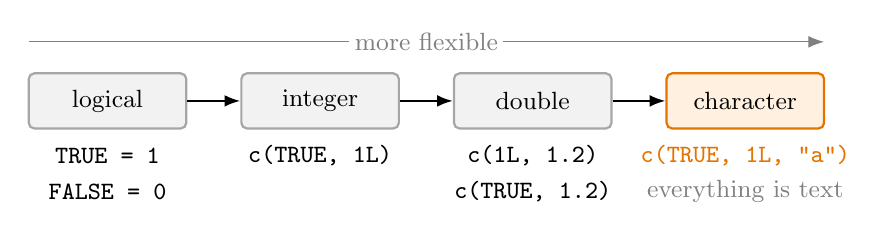
\begin{tikzpicture}[font=\small, >={Latex[length=2mm]},
  type/.style={draw, thick, rounded corners=2pt, minimum width=20mm, minimum height=7mm, inner sep=1pt},
  ex/.style={font=\small\ttfamily}]
  \node[type, gray!70, fill=gray!10, text=black] (l) at (1.0,0) {logical};
  \node[type, gray!70, fill=gray!10, text=black] (i) at (3.7,0) {integer};
  \node[type, gray!70, fill=gray!10, text=black] (d) at (6.4,0) {double};
  \node[type, orange!90!black, fill=orange!12, text=black] (c) at (9.1,0) {character};
  \draw[->, thick] (l) -- (i);
  \draw[->, thick] (i) -- (d);
  \draw[->, thick] (d) -- (c);
  \draw[->, gray] (0.0,0.75) -- (10.1,0.75);
  \node[gray, fill=white, inner sep=2pt] at (5.05,0.75) {more flexible};
  \node[ex] at (1.0,-0.7) {TRUE = 1};
  \node[ex] at (1.0,-1.15) {FALSE = 0};
  \node[ex] at (3.7,-0.7) {c(TRUE, 1L)};
  \node[ex] at (6.4,-0.7) {c(1L, 1.2)};
  \node[ex] at (6.4,-1.15) {c(TRUE, 1.2)};
  \node[ex, orange!90!black] at (9.1,-0.7) {c(TRUE, 1L, "a")};
  \node[gray] at (9.1,-1.15) {everything is text};
\end{tikzpicture}
\end{document}
